\documentclass{beamer}
\usepackage[utf8]{inputenc}
\usepackage{xcolor}
\usepackage[T1]{fontenc}
\usepackage[normalem]{ulem}
\usepackage{graphicx}
\usetheme{Antibes}

\title{Analyse comparée d'arbres taxonomiques}
\author{C. \textsc{Réda}\\sous la direction de M. \textsc{Nikolski} \& M. \textsc{Raffinot}}
\institute{CGFB, équipe CBIB, Bordeaux}
\date{du 1er juin au 27 juillet 2016}

\begin{document}
\maketitle
\tableofcontents
\setlength{\parindent}{1cm}

\addtobeamertemplate{footline}{\insertframenumber / \inserttotalframenumber}

\section{Déroulement du stage}

\begin{frame}
\tableofcontents[currentsection]
\end{frame}

\subsection{Lieu et modalités du stage}

\begin{frame}
\tableofcontents[currentsubsection]
\end{frame}

\begin{frame}
\frametitle{Informations sur le stage}

\begin{center}

\includegraphics[scale=0.3]{Images/bioinformatique.png}

\begin{itemize}
\item \uline{Lieu :} 
\begin{flushcenter} \bf Centre de Génomique Fonctionnelle \end{flushcenter}
\bigskip
\begin{flushcenter} (CGFB) \end{flushcenter}
\item \uline{Equipe :} 
\begin{flushcenter} \bf Centre de BioInformatique \end{flushcenter}
\bigskip
\begin{flushcenter} (CBIB) \end{flushcenter}
\item \uline{Dates :} 
\begin{flushcenter} du $1^{er}$ juin au 27 juillet 2016 \end{flushcenter}
\end{itemize}

\end{center}

%Une petite équipe d'une dizaine de personnes, informaticiens et biologistes, dans une plateforme de biologie qui propose des prestations et des projets recherche et développement
%lien avec MaBioVis au LaBRI et avec l'hôpital des enfants Pellegrin (à côté) de Bordeaux

\end{frame}

\subsection{Organisation}

\begin{frame}
\tableofcontents[currentsubsection]
\end{frame}

\begin{frame}
\frametitle{Projets de l'équipe CBIB}

\begin{itemize}
\item Une dizaine de logiciels de bioinformatique, dont \alert{Tango};
%TANGO dont le développement est à l'origine du stage
\pause
\item Participation et $3^{eme}$ place au concours international
\begin{flushcenter}\bf Dream Challenge \end{flushcenter};
%Concours international organisé par le National Cancer Institute (NCI), IBM Research, Sage Bionetworks et la International Society for Computational Biology (ISCB) qui vise à améliorer les logiciels d'analyse des tumeurs.

\begin{center}
\includegraphics[scale=0.1]{Images/dreamchallenge.png}
\end{center}

\pause
\item Participation au projet
\begin{flushcenter}\bf Galaxy \end{flushcenter};
%Système de fouille et de gestion de données bioinformatique
\pause
\item Collaborations avec :
     \begin{itemize}
     \item 
      \begin{flushcenter} l'\bf Inra\end{flushcenter} de Bordeaux, 
     \pause
     \item 
     \begin{flushcenter} le \bf LaBRI\end{flushcenter}, 
     \pause
     \item  
     \begin{flushcenter} \bf GenoToul Bioinformatique\end{flushcenter} à Toulouse, 
     \pause
     \item 
     \begin{flushcenter} et l'hôpital \bf Pellegrin\end{flushcenter} à Bordeaux.
     \end{itemize}
\end{itemize}

\end{frame}

\section{Sujet du stage}

%Le stage portait sur les arbres taxonomiques, qui sont des arbres représentant la classification des espèces dans des groupes selon leur histoire évolutive. En métagénomique, qui est l'étude du matériel génétique récupéré dans des environnements naturels, les arbres taxonomiques permettent d'identifier les espèces qui sont présentes dans l'échantillon recueilli, et d'alors déterminer la composition de la population présente dans l'environnement d'où provient l'échantillon.

%La métagénomique est un secteur très actif de nos jours en bioinformatique, grâce à la diminution des prix du traitement de l'ADN (via le séquençage) et au fait qu'elle permet l'étude d'espèces, en particulier de bactéries, non cultivables en laboratoire. Cette discipline a de nombreuses applications en biologie et en médecine.

%Le but de ce stage est d'améliorer l'analyse des données métagénomiques dans un cadre médical. Ici, nous nous concentrons sur l'analyse de l'ADN de bactéries présentes dans l'intestin humain.

\begin{frame}
\tableofcontents[currentsection]
\end{frame}

\subsection{Contexte scientifique}

\begin{frame}
\tableofcontents[currentsubsection]
\end{frame}

\begin{frame}
\frametitle{Traitement du matériel génétique brut}

%récupéré dans l'environnement naturel
\begin{itemize}
\item Extraction de l'ADN par réaction chimique;
\pause
\item Séquençage de l'ADN obtenu : obtention de la \alert{structure primaire} de l'ADN.
%L'ordre des ensembles de paires de bases construits avec la cytosine, l'adénine, la guanine et la thymine
\end{itemize}
\pause

\begin{block}{Next-Generation Sequencing (NGS)}
Méthode rapide, relativement bon marché de séquençage de l'ADN, encline aux erreurs. \\
Donne des morceaux de séquences (\alert{reads}) d'une longueur de 32 à 1 000 paires de bases.
\end{block}

\end{frame}

\begin{frame}
\frametitle{Identification des reads à des espèces}

\begin{itemize}
\item Séquençage réalisé sur les gènes 16S;
%Ces gènes contiennent des régions très conservées d'une bactérie à l'autre, et d'autres très variables. Ces dernières permettent d'identifier une bactérie.
\pause
\bigskip
\item Limites des \alert{régions hyper variables} difficiles à évaluer;
%Ce qui est source d'erreurs dans le séquençage.

\begin{center}
\includegraphics[scale=0.35]{Images/hypervariable.png}
\end{center}

\pause
\item \alert{Alignement} des reads obtenus sur ces régions à des séquences de référence.
%après séquençage
%En cas d'alignement optimal (avec une fonction de score maximisée ou minimisée), le read "matche" l'espèce correspondant à la séquence de référence.

\begin{center}
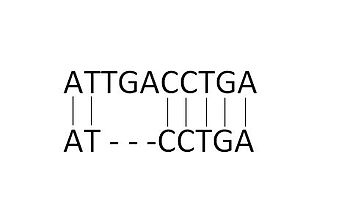
\includegraphics[scale=0.5]{Images/Sequence_gaps.JPG}
\end{center}

\end{itemize}

\end{frame}

\begin{frame}
\frametitle{Arbres taxonomiques}

\begin{block}{Arbre taxonomique} Graphe connexe acyclique non orienté de hauteur bornée, correspondant à l'histoire évolutive du monde vivant.
\end{block}

%Un arbre taxonomique est un arbre enraciné (= graphe connexe acyclique non orienté) de hauteur bornée. Dans la classification du projet GreenGenes, il existe 8 niveaux/générations appelés rangs taxonomiques. Le "premier" niveau correspond au monde vivant, le dernier niveau ne correspond qu'à une seule espèce vivante.

\begin{figure}
\subfigure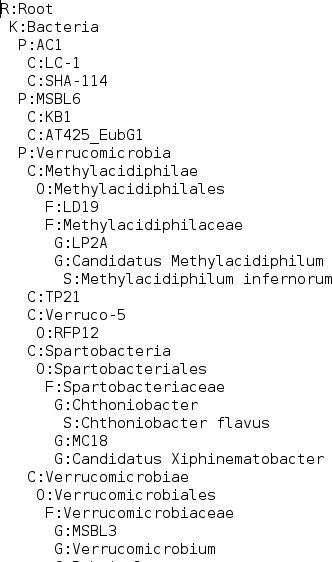
\includegraphics[scale=0.25]{Images/arbretaxo.png}
\subfigure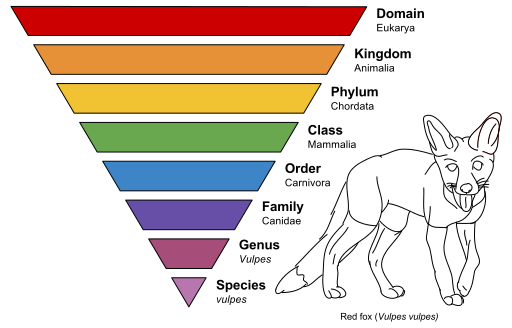
\includegraphics[scale=0.4]{Images/Taxonomic_Rank.png}
\end{figure}

%Il n'existe pas d'arbre taxonomique unique dans la communauté scientifique. Les classifications les plus utilisées sont celles de NCBI, GreenGenes et RDP. La hauteur de ces arbres, ainsi que les rangs taxonomiques, varient d'une base à l'autre.

\end{frame}

\begin{frame}
\frametitle{Arbres taxonomiques}

\begin{block}{Caractéristiques}
\begin{itemize}
\item Plus un noeud est proche de la racine, \\moins son degré est grand;
\item Nettement plus de feuilles que de noeuds internes;
%Pour l'arbre de GreenGenes réduit donné par TANGO, il y a 9 065 noeuds, dont 5 565 feuilles.
\item Assignation d'un \alert{read} plus complexe qu'il n'y paraît.
%Un read peut matcher plusieurs séquences de référence, donc plusieurs espèces. Cependant, il ne peut être assigné qu'à une seule espèce. En général, le read est alors assigné au LCA des espèces matchées, qui peut avoir un rang supérieur à S. Mais il existe des algorithmes améliorant cette assignation.
%De plus, il peut exister des erreurs dans le séquençage et donc dans le matching.
\end{itemize}
\end{block}

\end{frame}

\begin{frame}

\begin{alertblock}{Least Common Ancestor (LCA) de A et B}
Dernier noeud de la partie commune des chemins de la racine jusqu'à A et B.
\end{alertblock}

\bigskip

\begin{center}
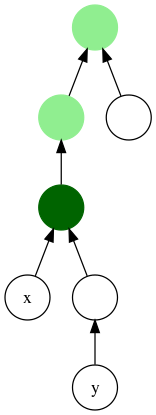
\includegraphics[scale=0.35]{Images/Lowest_common_ancestor.png}
\end{center}

\end{frame}

\begin{frame}
\frametitle{Problématiques de la métagénomique}

Existence d'algorithmes :
\pause
\begin{itemize}
\item améliorant l'alignement des reads aux séquences (Smith et Waterman, 1981);
\pause
\item améliorant l'assignation dans l'arbre des reads matchés (Clemente et al., 2011 : l'outil\textsc{ \bf Tango});
\pause
\item implémentant des mesures quantifiant la pertinence d'un arbre taxonomique (Robinson et Foulds, 1981)
\item ...
\end{itemize}
\pause

\begin{center}
Mais...
\end{center}
%Il manque des outils pour comparer les données métagénomiques en fonction d'informations non taxonomiques (ou métadonnées), ou trouver les critères non taxonomiques qui discriminent les échantillons dans un certain ensemble de départ.

%Par exemple, pour des patients atteints de mucovisidose, étant donné des échantillons de leurs flores intestinales, on souhaite savoir si les flores de patients traités par antibiotique sont différentes (et si oui, en quoi) des flores des patients sans traitement.

%Ces questions sont traitées pour le moment par analyse statistique, mais il manque un outil de traitement semi-automatique d'interprétation des données métagénomiques.

\end{frame}

\subsection{Problèmes}

\begin{frame}
\tableofcontents[currentsubsection]
\end{frame}

\begin{frame}
\frametitle{Problème des paires les plus dissemblables}

%Les fichiers d'entrée communs à tous les problèmes étaient l'arbre taxonomique de GreenGenes, une numérotation fixée des échantillons de patients, des bactéries et des métadonnées, et une matrice donnant les valeurs numériques de chaque métadonnée pour chaque échantillon.
\uline{Entrée :} \begin{itemize} \item Une matrice d'occurrence des assignations dans les échantillons. \end{itemize}

\bigskip
\uline{Sortie :} L'ensemble des paires d'échantillons les plus dissemblables.

\end{frame}

%Deux problèmes qui déterminent l'existence d'une correspondance entre métadonnées et populations bactériennes

\begin{frame}
\frametitle{Problème de compatibilité de la classification}

\uline{Entrée :} \begin{itemize} \item Un sous-ensemble N de noeuds/bactéries; \item Un tableau contenant les noeuds matchés dans chaque échantillon; \item Un sous-ensemble M de métadonnées. \end{itemize}

\bigskip
\uline{Sortie :} Existe-t-il une correspondance entre N et M ?

%La classification des échantillons selon la valeur des métadonnées du sous-ensemble correspond-elle à la classification des échantillons selon leurs populations bactériennes restreintes au sous-ensemble de noeuds choisis ?

\end{frame}

\begin{frame}
\frametitle{Problème de meilleure classification}

\uline{Entrée :} \begin{itemize} \item Un tableau contenant les noeuds matchés dans chaque échantillon; \item Un sous-ensemble de métadonnées M. \end{itemize}

\bigskip
\uline{Sortie :} Un sous-ensemble N de noeuds tel que N ait une correspondance avec M.

%Un ensemble de noeuds qui donne la meilleure discrimination entre les échantillons par rapport à la classification par rapport aux métadonnées du sous-ensemble.

\end{frame}

\section{Travail de recherche}

\begin{frame}
\tableofcontents[currentsection]
\end{frame}

\subsection{Méthode pseudo-statistique (résumé)}

\begin{frame}
\tableofcontents[currentsubsection]
\end{frame}

\begin{frame}
\frametitle{Rappel des problèmes}

\begin{itemize}
\item \begin{flushcenter} \bf Problème des paires les plus dissemblables\end{flushcenter}\\ \uline{Sortie :} L'ensemble des paires d'échantillons les plus dissemblables.
\item \uncover<->{ \begin{flushcenter} \bf Problème de compatibilité de la classification\end{flushcenter}\\ \uline{Sortie :} Existe-t-il une correspondance entre N et M ?}
\item \uncover<->{ \begin{flushcenter} \bf Problème de meilleure classification\end{flushcenter}\\ \uline{Sortie :} Un sous-ensemble N de noeuds tel que N ait une correspondance avec M.}
\end{itemize}

%Une méthode qui utilise des mesures sur les populations bactériennes (donc sur les arbres taxonomiques induits par les échantillons), indépendante des métadonnées, pour donner une distance entre les échantillons pour résoudre le problème des paires les plus dissemblables. Cette méthode utilise directement la sortie de TANGO, et donc l'assignation des noeuds dans les échantillons. L'outil associé TAXOTREE peut être considéré comme un outil d'interprétation de TANGO.

%Par manque, on ne parlera que de manière succincte de cette partie, moins intéressante que les deux autres.

\end{frame}

%\begin{frame}
%\frametitle{Méthode pseudo-statistique : définitions}

%\begin{block}{Arbre taxonomique induit par un échantillon}
%Forêt de sous-arbres de l'arbre taxonomique de référence constitués des seuls noeuds assignés dans l'échantillon.
%\end{block}
%\pause
%*dessin*

%\begin{block}{Motif de l'arbre taxonomique (induit)}
%Sous-graphe connexe de l'arbre taxonomique (induit).
%\end{block}

%*dessin*

%\begin{block}{Classes d'échantillons induites par une métadonnée}
%Ensemble de groupes d'échantillons disjoints, non vides, selon la valeur numérique -connue- de la métadonnée.
%\end{block}

%*exemple*

%\end{frame}

%\begin{frame}
%\frametitle{Mesures utilisées dans \textsc{\bf TaxoTree} (1)}

%\begin{block}{Total Ratio}
%\begin{center}
%$TR(G_{1},G_{2}) = \frac{n}{n_{1} + n_{2} + n}$
%\end{center}
%\end{block}

%G1, G2 sont deux sous-ensembles d'échantillons
%n est le nombre d'assignations aux noeuds communs aux échantillons de G1 et G2 (noeuds qui sont assignés au moins dans un échantillon de G1 et au moins dans un échantillon de G2)
%ni est le nombre d'assignations aux noeuds assignés seulement dans un échantillon de Gi
%S'intéresse aux populations de noeuds

%\begin{figure}
%\centering
%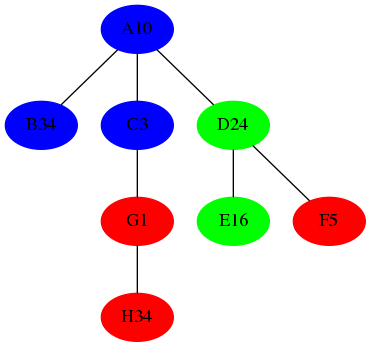
\includegraphics[scale=0.3]{Images/totalratio.png}
%\caption{$TR$ = $\frac{10 + 3 + 34}{(1 + 34 + 5) + (10 + 3 + 34) + (24 + 16)} \simeq 0.37$}
%\end{figure}

%\end{frame}

%\begin{frame}
%\frametitle{Mesures utilisées dans \textsc{\bf TaxoTree} (2)}

%\begin{block}{Pattern Ratio}
%\begin{center}
%$PR(G_{1},G_{2}) = \frac{n_{common}}{n_{specific}}$
%\end{center}
%\end{block}

%Un motif commun à deux groupes d'échantillons est un sous-graphe connexe commun aux arbres taxonomiques induits par G1 et G2.

%G1, G2 sont deux sous-ensembles d'échantillons
%n est le nombre d'assignations aux noeuds d'un motif commun (de taille > 1) dans les arbres induits par G1 et G2.
%N est le nombre d'assignations dans les motifs spécifiques à G1 et dans les motifs spécifiques à G2.

%\begin{figure}
%\centering
%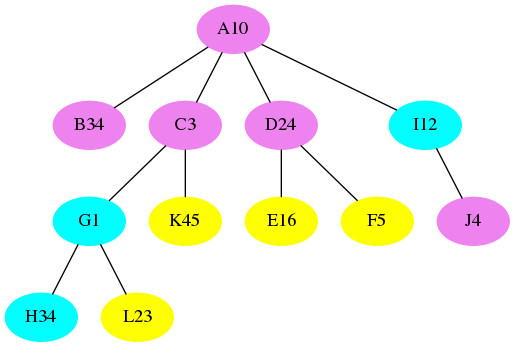
\includegraphics[scale=0.3]{Images/patternratio.png}
%\caption{$PR$ = $\frac{10 + 34 + 3 + 24}{(1 + 34 + 12) + (23 + 45 + 16 + 5)} \simeq 0.52$}
%\end{figure}

%Se concentre sur la proximité phylogénétique des noeuds des groupes d'échantillons. Cela correspond au "noyau fonctionnel" des bactéries de l'intestin, c'est-à-dire l'ensemble de bactéries nécessaire et suffisant pour faire fonctionner le système digestif.

%\end{frame}

%\begin{frame}
%\frametitle{Mesures utilisées dans \textsc{\bf TaxoTree} (3)}

%\begin{block}{Microbial Diversity}
%\begin{center}
%$MD(G) = \frac{n_{nodes}}{n_{tree}}$
%\end{center}
%\end{block}

%G est un sous-ensemble d'échantillons
%nnodes est le nombre de noeuds dans l'arbre induit par G
%ntree est le nombre de noeuds dans l'arbre taxonomique complet

%\begin{figure}
%\centering
%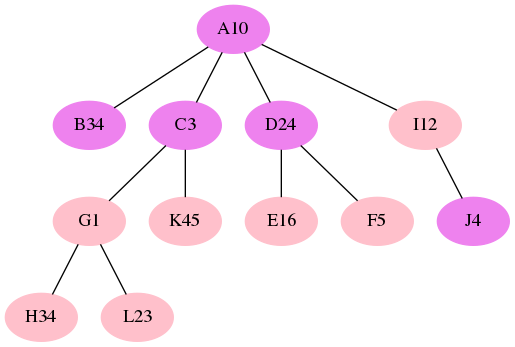
\includegraphics[scale=0.3]{Images/diversity.png}
%\caption{MD = \frac{5}{12} \simeq 0.42}
%\end{figure}

%La diversité bactérienne dans l'intestin est le facteur de l'équilibre de cet écosystème fragile.

%\end{frame}

\begin{frame}
\frametitle{Distance calculée}

\begin{block}{Coefficient de similarité s}
\begin{itemize}
\item Si $MD(G_{1}) - MD(G_{2}) = 0$ : 
\begin{center}
$ s(G_{1},G_{2}) = TR(G_{1},G_{2}) + PR(G_{1},G_{2})$
\end{center}
\item Sinon : 
\begin{center}
$ s(G_{1},G_{2}) = TR(G_{1},G_{2}) + PR(G_{1},G_{2}) - | MD(G_{1}) - MD(G_{2}) |$
\end{center}
\end{itemize}
\end{block}

\pause

\begin{block}{Coefficient de similarité \overline{s}}
\begin{center}
$\overline{s}(G_{1},G_{2}) = \frac{s(G_{1},G_{2}) - E(s)}{\sigma(s)}$
\end{center}
\end{block}

%G1 et G2 sont des sous-ensembles d'échantillons

%Si n est le nombre de classes induites par une métadonnée, on calcule alors s pour chaque paire de classes et on retourne la liste des paires de classes telle que le coefficient de similarité soit inférieur à la valeur du premier quartile.
%On compare alors cette valeur au coefficient de similarité portant sur les valeurs numériques des métadonnées (sommes des coefficients de similarité entre toutes les paires d'échantillons dans des groupes différents, qui sont les sommes des différences en valeur absolue des valeurs de certaines métadonnées -choisies par l'utilisateur)

\uline{Problème :} trouver des mesures pertinentes !

%Caractériser les populations microbiennes sur quelques traits reste grossier, et les phénomènes biologiques mis en jeu ne sont pas connus complètement. Des hypothèses a priori sur ceux-ci sont donc nécessaires, ce qui peut biaiser le résultat final.

\end{frame}

\subsection{Apprentissage supervisé}

\begin{frame}
\tableofcontents[currentsubsection]
\end{frame}

\begin{frame}
\frametitle{Rappel des problèmes}

\begin{itemize}
\item \uncover<->{\begin{flushcenter} \bf Problème des paires les plus dissemblables\end{flushcenter}\\ \uline{Sortie :} L'ensemble des paires d'échantillons les plus dissemblables.}
\item \begin{flushcenter} \bf Problème de compatibilité de la classification\end{flushcenter}\\ \uline{Sortie :} Existe-t-il une correspondance entre N et M ?
\item \begin{flushcenter} \bf Problème de meilleure classification\end{flushcenter}\\ \uline{Sortie :} Un sous-ensemble N de noeuds tel que N ait une correspondance avec M.
\end{itemize}

%Une deuxième approche essaie d'identifier les noeuds de l'arbre taxonomique qui permettent de séparer les échantillons en groupes similaires à ceux obtenus en discriminant les échantillons selon les valeurs numériques de certaines métadonnées, ce qui sous-entend que la présence de ces noeuds est liée à ces métadonnées. Cette approche résout le problème de compatibilité de classification et de meilleure classification. Cette méthode, comme la suivante, néglige l'assignation par TANGO et se concentre sur la sortie de l'alignement des reads avec les séquences de référence, où un read peut être matché à plusieurs séquences de référence. On suppose que l'espèce associée au read est dans l'ensemble des espèces matchées...

\end{frame}

\begin{frame}
\frametitle{Quelques notions de\textsc{ \it Machine Learning }}

\begin{block}{\begin{flushcenter} \it Machine Learning \end{flushcenter}}
Paradigme qui automatise la reconnaissance de certains motifs.
\end{block}

%C'est-à-dire que l'ordinateur est capable de trier les données selon leur contenu, sans que le tri soit explicitement programmé. Il permet de traiter de grosses masses de données.

%Utilisé notamment dans la repérage de spams dans les boîtes mail : le programme identifie des mots souvent utilisés dans les emails malveillants ("amour", "bonheur", "fortune") dans les mails de la boîte de réception. Il calcule alors la probabilité que le mail considéré soit non-malveillant sachant qu'il a un telle proportion de ces mots-clés. Si celle-ci est inférieure à celle qu'il soit un spam sachant qu'il a cette proportion de mots-clés, le mail est alors considéré comme un spam. Pour calculer ces probabilités, un ensemble de départ de mails identifiés comme spams et sains est donné au programme pour "l'entraînement". A l'inverse, un programme sans Machine Learning aurait besoin par exemple d'un seuil de fréquences d'apparition des mots-clés (à choisir...) pour pouvoir identifier les spams.

%L'une des plus grandes catégories d'algorithmes de Machine Learning est l'apprentissage supervisé.

\pause

\begin{block}{Apprentissage supervisé}
Classification des données dans des catégories \alert{fixées}, avec une connaissance\textsc{ \it a priori} acquise sur un \alert{ensemble d'entraînement}.
\end{block}

%l'exemple des mails. L'un des types de classificateurs les plus utilisés est le classificateur naïf bayésien.

\end{frame}

\begin{frame}
\frametitle{Le classificateur naïf bayésien}

\begin{block}{Classificateur naïf bayésien}
Pour $k$ classes disjointes de données $(C_{i})_{1 \le i \le k}$, des critères $(F_{i})_{1 \le i \le m}$, et une donnée $d$ à classer, ayant $(F_{i} = x_{i})_{1 \le i \le m}$,\\ La classe de $d$ est la classe $C_{j}$ telle que:\\
\begin{center}
$P(C_{j} | F_{1} = x_{1}, ..., F_{m} = x_{m})$\\
$= \max_{h \in \{ 1, ..., k \}}P(C_{h} | F_{1} = x_{1}, ... F_{m} = x_{m})$.\\
\end{center}
\end{block}

%Ce classificateur utilise de nombreuses hypothèses a priori pour calculer ces probabilités, comme l'indépendance entre les valeurs numériques des métadonnées.

\end{frame}

\begin{frame}
\frametitle{Calcul de la pertinence de la classification obtenue}

%Ce coefficient calcule la pertinence de la classification pour résoudre le problème de la meilleure classification.

\begin{block}{Coefficient J de Youden}
$J(C) = \frac{TP(C)}{TP(C) + FN(C)} + \frac{TN(C)}{TN(C) + FP(C)} - 1$.
\end{block}

\begin{figure}
\centering
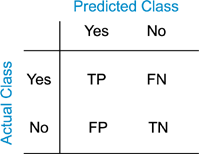
\includegraphics[scale=0.40]{Images/confusionmatrix.png}
\end{figure}

%True Positive TP : données qui appartiennent à C et qui ont été assignées à C par le classificateur
%True Negative TN : données qui n'appartiennent pas à C et qui n'ont pas été assignées à C
%False Negative FN : données qui appartiennent à C et qui n'ont pas été assignées à C
%False Positive FP : données qui n'appartiennt pas à C et qui ont été assignées à C

%Quand $J(C) = 1$, la classification est parfaite; pas de FN et de FP
%Quand $J(C) = 0$, la classification ne fait pas mieux qu'un classificateur aléatoire;
%Quand $J(C) = -1$, la classification est totalement fausse. pas de TN et de TP

%D'après ce qui précède, la meilleure classification est telle que pour chaque classe, le coefficient J de Youden est le plus proche de 1.

\pause

\begin{block}{Coefficient \alert{modifié} pour $k$ classes $(C_{i})_{1 \le i \le k}$}
\begin{center}
Classification "optimale" : $k - \sum{_{i = 1}^{k}}{J(C_{i})}$ minimal, positif.
\end{center}
\end{block}

\end{frame}

\begin{frame}
\frametitle{Le \textsc{\bf TaxoClassifier} : étapes d'une classification}

Etant donnés un ensemble de métadonnées M (et donc des classes induites par M) et de noeuds N :
\pause
\bigskip
\begin{enumerate}
\item \alert{Entraînement} du classificateur;
%Choix aléatoire d'un sous-ensemble strict R de l'ensemble des échantillons pour l'entraînement
%Calcul de la probabilité d'avoir un certain noeud de N pour un échantillon
%Comptage et identification des noeuds matchés, appartenant à N, dans chaque échantillon
\pause
\item Pour chaque échantillon non assigné, calcul des \alert{probabilités postérieures} à chaque classe;
%Les probabilités présentées précédemment
\end{enumerate}
\end{frame}

\begin{frame}
\frametitle{Le classificateur naïf bayésien}
\begin{block}{Classificateur naïf bayésien}
\uncover<->{Pour $k$ classes disjointes de données $(C_{i})_{1 \le i \le k}$, des critères $(F_{i})_{1 \le i \le m}$, et une donnée $d$ à classer, ayant $(F_{i} = x_{i})_{1 \le i \le m}$,\\ La classe de $d$ est la classe $C_{j}$ telle que:\\}
\begin{center}
\alert{$P(C_{j} | F_{1} = x_{1}, ..., F_{m} = x_{m})$\\
$= \max_{h \in \{ 1, ..., k \}}P(C_{h} | F_{1} = x_{1}, ... F_{m} = x_{m})$}.\\
\end{center}
\end{block}
\end{frame}

\begin{frame}
\frametitle{Le \textsc{\bf TaxoClassifier} : étapes d'une classification}

Etant donnés un ensemble de métadonnées M (et donc des classes induites par M) et de noeuds N :
\bigskip
\begin{enumerate}
\item \alert{Entraînement} du classificateur;
\item Pour chaque échantillon non assigné, calcul des \alert{probabilités postérieures} à chaque classe;
\item Assignation de chaque échantillon à la classe qui maximise la probabilité précédente;
\pause
\item Retour du coefficient J de Youden \alert{modifié} associé à cette classification.
\pause
\end{enumerate}

\bigskip

\uline{Problème(s) :} Beaucoup d'hypothèses \textsc{\it a priori}, et de petites améliorations nécessaires pour gérer les cas limites !

\end{frame}

\subsection{Apprentissage non supervisé}

\begin{frame}
\tableofcontents[currentsubsection]
\end{frame}

\begin{frame}
\frametitle{Rappel des problèmes}

\begin{itemize}
\item \uncover<->{ \begin{flushcenter} \bf Problème des paires les plus dissemblables\end{flushcenter}\\ \uline{Sortie :} L'ensemble des paires d'échantillons les plus dissemblables.}
\item \uncover<->{\begin{flushcenter} \bf Problème de compatibilité de la classification\end{flushcenter}\\ \uline{Sortie :} Existe-t-il une correspondance entre N et M ?}
\item \begin{flushcenter} \bf Problème de meilleure classification\end{flushcenter}\\ \uline{Sortie :} Un sous-ensemble N de noeuds tel que N ait une correspondance avec M.

%La troisième méthode, associé à l'outil TaxoCluster, utilise l'apprentissage non supervisé, qui est un autre pan du Machine Learning. Elle consiste à diviser l'ensemble des échantillons en groupes d'échantillons les plus proches, en utilisant une distance ne dépendant que des populations bactériennes matchées, et à comparer les groupes obtenus (des clusters) avec les groupes obtenus en ne considérant que les valeurs numériques des métadonnées. 
\end{itemize}

\end{frame}

\begin{frame}
\frametitle{Notion de clustering}

%Une deuxième grande catégorie de Machine Learning est l'apprentissage non supervisé.

\begin{block}{Apprentissage non supervisé}
Identification des différentes classes de données, en étudiant la similarité entre les données.
\end{block}

\pause

%Un des algorithmes les plus connus de cette catégorie est l'algorithme des K-moyennes, qui est un algorithme de clustering.

\begin{block}{Clustering}
Partition d'un ensemble de données, telle que :
\begin{itemize} 
\item les parties obtenues \alert{minimisent} la distance entre les objets d'un même groupe;
\item la \alert{maximisent} entre les objets de deux groupes différents.
\end{itemize}
\end{block}

\end{frame}

\begin{frame}
\frametitle{Problème de clustering}

\begin{alertblock}{Complexité du problème de partition en k \textsc{\it clusters} de $n$ éléments}
Le problème de $k$-partition de $n$ éléments est NP-complet.
\end{alertblock}

\pause

\begin{block}{Etapes de l'algorithme des K-moyennes}
\begin{enumerate}
\item Initialisation des $k$ clusters
\item Tant que les clusters sont modifiés pendant la boucle
       \begin{itemize}
       \item Pour tout élément e de l'ensemble de départ
             \begin{itemize}   
             \item Déterminer le cluster C qui minimise la distance entre e et sa moyenne
             \item Affecter e à C
             \item Recalculer la moyenne de C
             \end{itemize}
       \end{itemize}
\end{enumerate}
\end{block}

%L'algorithme des K-moyennes ne garantit pas l'optimalité, ni la terminaison en temps raisonnable. Cependant, en pratique, il est rapide et permet de répondre à ce problème.

%Après choix de k et l'initialisation des k clusters avec un élément de l'ensemble de départ, l'algorithme calcule pour chaque élément e restant, et pour tout cluster C, la distance entre e et la moyenne du cluster C, c'est-à-dire l'élément "au centre" du cluster (en utilisant la distance donnée). e est alors attribué au cluster qui minimise cette distance, et la moyenne de ce cluster est alors recalculée avant d'itérer la boucle, jusqu'à convergence de la solution (les clusters restent les mêmes dune itération à l'autre).

\end{frame}

\begin{frame}
\frametitle{Notations utilisées dans \textsc{\bf TaxoCluster}}

Soit $T$ l'arbre taxonomique complet. Pour un certain read $i$ :
\begin{itemize}
\item $M_{i}$, ensemble de feuilles matchées par $i$;
\pause
\item $T_{i}$, sous-arbre de $T$ enraciné au LCA des feuilles de $M_{i}$;
\pause
\item $L_{i}$, ensemble des feuilles de $T_{i}$;
\pause
\item $N_{i}$, tel que $L_{i} = M_{i} \sqcup N_{i}$.
\pause
\end{itemize}

\begin{center}
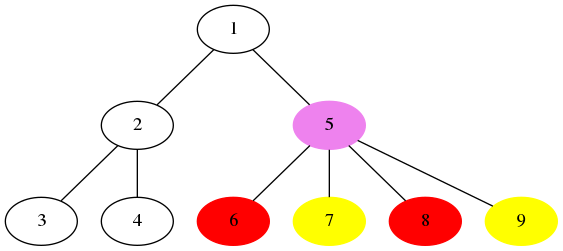
\includegraphics[scale=0.3]{Images/timili.png}
\end{center}

\end{frame}

\begin{frame}
\frametitle{Distances utilisées dans \textsc{\bf TaxoCluster}}

\begin{block}{"Distance des ensembles de matches"}
Pour deux reads $i$ et $j$,\\
\begin{center} $d_{matched}(i,j) = |M_{i}| + |M_{j}| - 2*|M_{i} \cap M_{j}|$. \end{center}
\end{block}

%Il est facile de vérifier que dmatched satisfait l'inégalité triangulaire, est symétrique et positive.
%La seule relation d'égalité valable entre les reads est celle des ensembles de match ici, car le noeud réellement associé à un read donné ne peut pas être connu, et on ne distingue pas les reads provenant d'une même espèce.
\pause

\begin{block}{"Distance de l'arbre de consensus"}
Pour deux reads $i$ et $j$, et un paramètre $q \in [0;1]$,
\begin{center}$d_{consensus}(i,j) = |L_{i}| + |L_{j}| - q*(|N_{i}\cap M_{j}| + |N_{j} \cap M_{i}|) - |M_{i} \cap M_{j}|$.\end{center}
\end{block}

%Il est facile de vérifier que c'est bien une distance. Le choix de q correspond au choix d'un arbre de consensus entre les deux arbres taxonomiques Ti et Tj : si q = 0, on considère un arbre de consensus strict, en ne gardant que les feuilles matchées dans les deux reads. Si q = 1, on conserve toutes les feuilles qui sont matchées dans l'un au moins des deux reads.

\end{frame}

\begin{frame}
\frametitle{Distance de l'arbre de consensus}

\begin{figure}
\centering
\subfigure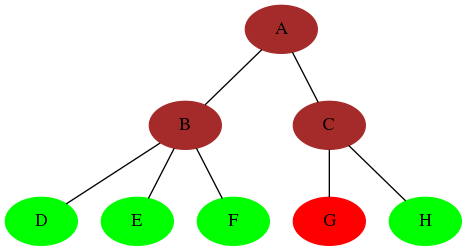
\includegraphics[scale=0.35]{Images/distance2-1.png}
\subfigure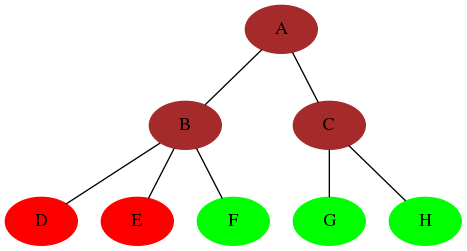
\includegraphics[scale=0.35]{Images/distance2-2.png}
%$M_{1}$ = \{D, E, F, H\} and $M_{2}$ = \{F, G, H\}
\caption{Quand $q = 0$, $d_{consensus}(T_{1},T_{2}) = 5 + 5 - 0 - 2 = 8$.\\Quand $q = 1$, $d_{consensus}(T_{1},T_{2}) = 5 + 5 - 1 \times (1 + 2) - 2 = 5$}
\end{figure}

\end{frame}

\begin{frame}
\frametitle{Le programme \textsc{\bf TaxoCluster}}

%Le principe essentiel de TaxoCluster est proche de celui de la précédente méthode : comparer le clustering réalisé sur les populations microbiennes et celui réalisé en ne considérant que les valeurs numériques des métadonnées pour faire ressortir une correspondance entre la flore intestinale et les métadonnées.

%Ceci explique que le k qui sera utilisé dans l'algorithme des K-moyennes sera en fait le nombre de classes induites par l'ensemble de métadonnées choisi. On initialise les clusters avec un échantillon appartenant à la classe (en regardant les valeurs de ses métadonnées), ce qui permet de régler deux problèmes de l'application de l'algorithme des K-moyennes.

\begin{enumerate}
\item Application de l'algorithme des K-moyennes avec $d_{matched}$
\bigskip
\pause
\item Suppression des éléments les moins pertinents 
%les plus éloignés des autres dans chaque cluster : on supprime les éléments dont la somme des distances aux autres points est supérieure au troisième quartile de la liste des distances
\bigskip
\pause
\item Application de l'algorithme des K-moyennes avec $d_{consensus}$
\bigskip
\pause
\item Comparaison des \alert{clusters} obtenus avec ceux induits par les métadonnées
%Obtention d'un coefficient entre 0 et 1, 1 étant l'adéquation parfaite entre les clusters
%Cela impliquerait peut-être une correspondance entre les populations et les métadonnées
%Le programme retourne aussi la liste des bactéries en commun dans chaque cluster (Note : assez grande en pratique : compter le nombre de matches ?)
\end{enumerate}

\end{frame}

\section{Evaluation des méthodes}

\begin{frame}
\tableofcontents[currentsection]
\end{frame}

\subsection{Implémentation}

\begin{frame}
\tableofcontents[currentsubsection]
\end{frame}

\begin{frame}
\frametitle{Implémentation}

\begin{itemize}
\item Implémentés en Python 2.9.7;
\bigskip
\pause
\item Disponibles sur GitHub;
\bigskip
\pause
\item \textsc{\bf TaxoCluster} et \textsc{\bf TaxoClassifier} encore en développement.
\end{itemize}

\end{frame}

\subsection{Evaluation}

\begin{frame}
\tableofcontents[currentsubsection]
\end{frame}

\begin{frame}
\frametitle{Evaluation}

\begin{itemize}
\item Evaluation en comparant les résultats obtenus par les différents logiciels et les résultats statistiques de l'étude de l'hôpital Pellegrin;
%décrire le contexte
\bigskip
\pause
\item Résultats donnés par \textsc{\bf TaxoTree} (première méthode) confirmant les résultats statistiques;
\bigskip
\pause
\item Manque de temps pour les tests de \textsc{\bf TaxoClassifier} et \textsc{\bf TaxoCluster}.
%expliquer le problème du parsing
\bigskip
\pause
\item En théorie : méthode de \textsc{TaxoCluster} meilleure que les autres;
%Pas d'hypothèses a priori, mais ne répond qu'à un seul des problèmes, contrairement à TaxoClassifier
\bigskip
\pause
\item En théorie : pire complexité temporelle pour \textsc{\bf TaxoCluster} (pire cas).
%En pratique, les trois programmes tournent entièrement en temps raisonnable sur un ordinateur de puissance moyenne.
\end{itemize}

\end{frame}

\section{Conclusion}

\begin{frame}
\tableofcontents[currentsection]
\end{frame}

\begin{frame}
\frametitle{Bilan et perspectives}

\begin{enumerate}
\item Propositions de trois méthodes pour répondre au(x) problème(s);
\bigskip
\pause
\item Utilisables sur un ordinateur de puissance moyenne;
\bigskip
\pause
\item Nécessité d'autres tests.
%Etude plus approfondie de l'interprétation biologique (cohérence). Résultats dépendent des traitements préalables sur les valeurs numériques (normalisation, standardisation du protocole, ...)
\end{enumerate}

\end{frame}

\section{Bibliographie}
\begin{frame}
\frametitle{Sources}

\begin{itemize}
\item \textsc{ \bf Flexible taxonomic assignment of ambiguous sequencing}, J. Clemente, J. Jansson et G. Valiente, \textsc{ \it BMC Bioinformatics}, 2011.
\item \textsc{\bf Impact de l'antibiothérapie sur le microbiote intestinal chez l'enfant atteint de mucovisidose}, R. Enaud, \textsc{\it Université de Bordeaux, CHU Pellegrin}, 2016.
\item \textsc{\bf Understanding Machine Learning: From Theory to Algorithms}, S. Shalev-Shwartz et S. Ben-David, \textsc{\it Cambridge University Press}, 2014.
\item ...
\end{itemize}

\end{frame}

\end{document}
